\documentclass[8pt,aspectratio=169]{beamer}
\usetheme{Madrid}
\usepackage{graphicx}
\usepackage{booktabs}
\usepackage{adjustbox}
\usepackage{multicol}
\usepackage{amsmath}
\usepackage{tikz}
\usetikzlibrary{shapes,arrows,positioning}

% Color definitions
\definecolor{mlblue}{RGB}{0,102,204}
\definecolor{mlpurple}{RGB}{51,51,178}
\definecolor{mllavender}{RGB}{173,173,224}
\definecolor{mllavender2}{RGB}{193,193,232}
\definecolor{mllavender3}{RGB}{204,204,235}
\definecolor{mllavender4}{RGB}{214,214,239}
\definecolor{mlorange}{RGB}{255, 127, 14}
\definecolor{mlgreen}{RGB}{44, 160, 44}
\definecolor{mlred}{RGB}{214, 39, 40}
\definecolor{mlgray}{RGB}{127, 127, 127}

% Paradigm-specific colors
\definecolor{supervisedblue}{RGB}{0,102,204}
\definecolor{unsupervisedgreen}{RGB}{34,139,34}
\definecolor{reinforcementorange}{RGB}{255,100,0}

% Additional colors
\definecolor{lightgray}{RGB}{240, 240, 240}
\definecolor{midgray}{RGB}{180, 180, 180}

% Apply custom colors to Madrid theme
\setbeamercolor{palette primary}{bg=mllavender3,fg=mlpurple}
\setbeamercolor{palette secondary}{bg=mllavender2,fg=mlpurple}
\setbeamercolor{palette tertiary}{bg=mllavender,fg=white}
\setbeamercolor{palette quaternary}{bg=mlpurple,fg=white}

\setbeamercolor{structure}{fg=mlpurple}
\setbeamercolor{section in toc}{fg=mlpurple}
\setbeamercolor{subsection in toc}{fg=mlblue}
\setbeamercolor{title}{fg=mlpurple}
\setbeamercolor{frametitle}{fg=mlpurple,bg=mllavender3}
\setbeamercolor{block title}{bg=mllavender2,fg=mlpurple}
\setbeamercolor{block body}{bg=mllavender4,fg=black}

% Remove navigation symbols
\setbeamertemplate{navigation symbols}{}

% Clean itemize/enumerate
\setbeamertemplate{itemize items}[circle]
\setbeamertemplate{enumerate items}[default]

% Reduce margins for more content space
\setbeamersize{text margin left=5mm,text margin right=5mm}

% Command for bottom annotation
\newcommand{\bottomnote}[1]{%
\vfill
\vspace{-2mm}
\textcolor{mllavender2}{\rule{\textwidth}{0.4pt}}
\vspace{1mm}
\footnotesize
\textbf{#1}
}

\title{Machine Learning Paradigms}
\subtitle{Traditional vs AI-Based Approaches}
\author{Machine Learning Overview}
\institute{2025}
\date{\today}

\begin{document}

% ==================== TITLE SLIDE ====================
\begin{frame}[plain]
\titlepage
\end{frame}

% ==================== INTRODUCTION ====================
\begin{frame}[t]{Traditional vs Machine Learning Approaches}
\begin{columns}[T]
\column{0.48\textwidth}
\textbf{Traditional Programming}

Start with \textbf{explicit rules}:
\begin{itemize}
\item Experts encode domain knowledge as rules
\item Programmer implements decision logic
\item System follows predetermined instructions
\item Behavior is fully specified in code
\end{itemize}

\vspace{0.5em}
\textbf{Characteristics:}
\begin{itemize}
\item Transparent and interpretable
\item Works well for well-defined problems
\item Requires comprehensive domain expertise
\item Struggles with complex, nuanced patterns
\item Rules must be manually updated
\end{itemize}

\column{0.48\textwidth}
\textbf{Machine Learning}

Start with \textbf{data and examples}:
\begin{itemize}
\item Algorithms discover patterns from data
\item Rules emerge through learning process
\item System improves with more experience
\item Behavior learned, not programmed
\end{itemize}

\vspace{0.5em}
\textbf{Three Main Learning Paradigms:}
\begin{itemize}
\item \textcolor{supervisedblue}{\textbf{Supervised}} - Learn from labeled examples
\item \textcolor{unsupervisedgreen}{\textbf{Unsupervised}} - Find structure in unlabeled data
\item \textcolor{reinforcementorange}{\textbf{Reinforcement}} - Learn optimal actions through trial and error
\end{itemize}
\end{columns}

\bottomnote{Fundamental difference: Traditional = explicit programming, ML = learning from data}
\end{frame}

% ==================== WHAT IS MACHINE LEARNING? ====================
\begin{frame}[t]{What is Machine Learning?}
\begin{columns}[T]
\column{0.48\textwidth}
\textbf{Core Definition}

\vspace{0.3em}
``A computer program learns from experience E with respect to task T if its performance P improves with experience.'' --- Tom Mitchell

\vspace{0.5em}
\textbf{Key Concepts:}
\begin{itemize}
\item \textbf{Learning} = improving performance through experience
\item \textbf{Generalization} = performing well on new, unseen data
\item \textbf{Not memorization} = patterns, not examples
\end{itemize}

\vspace{0.5em}
\textbf{What ML Needs:}
\begin{itemize}
\item Data (the ``experience'')
\item Features (representation of data)
\item Learning algorithm
\item Performance metric
\end{itemize}

\column{0.48\textwidth}
\textbf{The Learning Process}

\vspace{0.3em}
\begin{enumerate}
\item \textbf{Collect data}: Gather examples and experiences
\item \textbf{Represent data}: Extract features (numbers, vectors)
\item \textbf{Split data}: Training, validation, testing
\item \textbf{Train model}: Learn patterns from training data
\item \textbf{Validate}: Tune parameters on validation data
\item \textbf{Test}: Evaluate on completely unseen test data
\end{enumerate}

\vspace{0.5em}
\textbf{Critical Insight:}

\textcolor{mlpurple}{\textbf{The goal is NOT to memorize training data, but to generalize to new situations.}}

Test performance measures true learning.
\end{columns}

\bottomnote{ML is fundamentally about pattern recognition and prediction from data, not rule following}
\end{frame}

% ==================== THE ML WORKFLOW ====================
\begin{frame}[t]{The Machine Learning Workflow}
\begin{center}
\includegraphics[width=0.75\textwidth,height=0.75\textheight,keepaspectratio]{ml_workflow.pdf}
\end{center}

\vspace{0.3em}
\textbf{Key Stages:} Data Collection → Preprocessing → Split (Train/Val/Test) → Train → Validate (iterate until good) → Test ONCE → Deploy → Monitor (retrain when needed)

\bottomnote{Critical: Iterative process with feedback loops - validation guides tuning, monitoring triggers retraining}
\end{frame}

% ==================== SUPERVISED LEARNING ====================
\begin{frame}[t]{\textcolor{supervisedblue}{Supervised Learning}: Learn from Labeled Examples}
\begin{columns}[T]
\column{0.58\textwidth}
\begin{center}
\includegraphics[width=0.98\textwidth,height=0.68\textheight,keepaspectratio]{traditional_vs_ml_supervised.pdf}
\end{center}

\column{0.38\textwidth}
\textbf{Core Idea:}

Learn mapping $f: X \rightarrow Y$ from labeled examples $(x_i, y_i)$

\vspace{0.5em}
\textbf{Two Main Types:}
\begin{itemize}
\item \textbf{Classification}: Predict discrete labels (cat/dog, spam/not spam)
\item \textbf{Regression}: Predict continuous values (price, temperature)
\end{itemize}

\vspace{0.5em}
\textbf{Requirements:}
\begin{itemize}
\item Large labeled dataset
\item Quality labels (expensive!)
\item Representative examples
\end{itemize}

\vspace{0.5em}
\textbf{When to Use:}
\begin{itemize}
\item Clear input-output relationship
\item Labels available
\item Prediction task
\end{itemize}

\vspace{0.5em}
\textbf{Evaluation:}

Accuracy, precision, recall, F1 (classification)

MSE, R$^2$, MAE (regression)
\end{columns}

\vfill
\vspace{-2mm}
\textcolor{mllavender2}{\rule{\textwidth}{0.4pt}}
\vspace{1mm}
\small
\textbf{Key insight: Model learns statistical patterns that correlate inputs with labels}
\end{frame}

% ==================== UNSUPERVISED LEARNING ====================
\begin{frame}[t]{\textcolor{unsupervisedgreen}{Unsupervised Learning}: Find Structure in Unlabeled Data}
\begin{columns}[T]
\column{0.58\textwidth}
\begin{center}
\includegraphics[width=0.98\textwidth,height=0.68\textheight,keepaspectratio]{traditional_vs_ml_unsupervised.pdf}
\end{center}

\column{0.38\textwidth}
\textbf{Core Idea:}

Discover patterns in data without labels or guidance

\vspace{0.5em}
\textbf{Main Techniques:}
\begin{itemize}
\item \textbf{Clustering}: Group similar data points (K-means, hierarchical)
\item \textbf{Dimensionality Reduction}: PCA, t-SNE, UMAP
\item \textbf{Anomaly Detection}: Find outliers
\item \textbf{Generative Models}: Learn data distribution
\end{itemize}

\vspace{0.5em}
\textbf{When to Use:}
\begin{itemize}
\item No labels available
\item Exploratory analysis
\item Data preprocessing
\item Understanding structure
\end{itemize}

\vspace{0.5em}
\textbf{Challenge:}

No objective ground truth for evaluation - requires domain knowledge to validate results
\end{columns}

\vfill
\vspace{-2mm}
\textcolor{mllavender2}{\rule{\textwidth}{0.4pt}}
\vspace{1mm}
\small
\textbf{Key: Finds statistical similarity in feature space, not semantic relationships}
\end{frame}

% ==================== REINFORCEMENT LEARNING ====================
\begin{frame}[t]{\textcolor{reinforcementorange}{Reinforcement Learning}: Learn Through Sequential Decisions}
\begin{columns}[T]
\column{0.48\textwidth}
\begin{center}
\includegraphics[width=0.95\textwidth,height=0.55\textheight,keepaspectratio]{traditional_vs_ml_reinforcement.pdf}
\end{center}

\vspace{0.3em}
\begin{center}
\textbf{The RL Loop:}

\includegraphics[width=0.90\textwidth,keepaspectratio]{rl_agent_environment_loop.pdf}
\end{center}

\column{0.48\textwidth}
\textbf{Core Idea:}

Agent learns policy $\pi(a|s)$ to maximize cumulative reward through trial-and-error

\vspace{0.5em}
\textbf{Key Components:}
\begin{itemize}
\item \textbf{State} $s$: Current situation
\item \textbf{Action} $a$: Possible choices
\item \textbf{Reward} $r$: Feedback signal
\item \textbf{Policy} $\pi$: Strategy to learn
\end{itemize}

\vspace{0.5em}
\textbf{When to Use:}
\begin{itemize}
\item Sequential decisions
\item Delayed rewards
\item Control problems
\item Game AI, robotics
\end{itemize}

\vspace{0.5em}
\textbf{Challenges:}
\begin{itemize}
\item Sample inefficient (needs many trials)
\item Credit assignment problem
\item Exploration vs exploitation
\item Reward function design critical
\end{itemize}
\end{columns}

\vfill
\vspace{-2mm}
\textcolor{mllavender2}{\rule{\textwidth}{0.4pt}}
\vspace{1mm}
\small
\textbf{Key: Agent-environment interaction is cyclic - actions affect future states}
\end{frame}

% ==================== SUPERVISED EXAMPLE WITH CATS/DOGS ====================
\begin{frame}[t]{\textcolor{supervisedblue}{Supervised Learning Example: Cat vs Dog Classification}}
\begin{columns}[T]
\column{0.48\textwidth}
\textbf{Traditional Approach}

Expert writes rules:
\begin{itemize}
\item IF pointy ears AND whiskers AND meows $\rightarrow$ CAT
\item IF floppy ears AND barks $\rightarrow$ DOG
\end{itemize}

\vspace{0.3em}
\begin{center}

\begin{tikzpicture}[scale=0.7]
% Simple cat representation
\fill[orange!80] (0,0) circle (0.8);
\fill[orange!60] (-0.5,0.6) -- (-0.3,1.2) -- (-0.1,0.6);
\fill[orange!60] (0.5,0.6) -- (0.3,1.2) -- (0.1,0.6);
\fill[white] (-0.3,0.1) circle (0.15);
\fill[white] (0.3,0.1) circle (0.15);
\fill[black] (-0.3,0.1) circle (0.08);
\fill[black] (0.3,0.1) circle (0.08);
\node[below] at (0,-1) {CAT};
\end{tikzpicture}
\end{center}

\column{0.48\textwidth}
\textbf{ML Approach}

\textbf{Step 1: Training}

\begin{center}
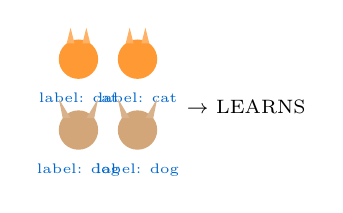
\begin{tikzpicture}[scale=0.5]
% Training cats
\fill[orange!80] (0,0) circle (0.5);
\fill[orange!60] (-0.3,0.4) -- (-0.2,0.8) -- (-0.1,0.4);
\fill[orange!60] (0.3,0.4) -- (0.2,0.8) -- (0.1,0.4);
\node[below,font=\tiny] at (0,-0.6) {\textcolor{supervisedblue}{label: cat}};

\fill[orange!80] (1.5,0) circle (0.5);
\fill[orange!60] (1.2,0.4) -- (1.3,0.8) -- (1.4,0.4);
\fill[orange!60] (1.8,0.4) -- (1.7,0.8) -- (1.6,0.4);
\node[below,font=\tiny] at (1.5,-0.6) {\textcolor{supervisedblue}{label: cat}};

% Training dogs
\fill[brown!70] (0,-1.8) circle (0.5);
\fill[brown!60] (-0.4,-1.5) -- (-0.5,-1) -- (-0.2,-1.5);
\fill[brown!60] (0.4,-1.5) -- (0.5,-1) -- (0.2,-1.5);
\node[below,font=\tiny] at (0,-2.4) {\textcolor{supervisedblue}{label: dog}};

\fill[brown!70] (1.5,-1.8) circle (0.5);
\fill[brown!60] (1.1,-1.5) -- (1,-1) -- (1.3,-1.5);
\fill[brown!60] (1.9,-1.5) -- (2,-1) -- (1.7,-1.5);
\node[below,font=\tiny] at (1.5,-2.4) {\textcolor{supervisedblue}{label: dog}};

\node[right,font=\scriptsize] at (2.5,-1.2) {$\rightarrow$ LEARNS};
\end{tikzpicture}
\end{center}

\vspace{0.3em}
\textbf{Step 2: Prediction}

\begin{center}
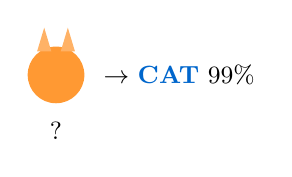
\begin{tikzpicture}[scale=0.6]
% New cat
\fill[orange!80] (0,0) circle (0.6);
\fill[orange!60] (-0.4,0.5) -- (-0.25,1) -- (-0.1,0.5);
\fill[orange!60] (0.4,0.5) -- (0.25,1) -- (0.1,0.5);
\node[below,font=\small] at (0,-0.8) {?};
\node[right,font=\small] at (0.8,0) {$\rightarrow$ \textcolor{supervisedblue}{\textbf{CAT}} 99\%};
\end{tikzpicture}
\end{center}
\end{columns}

\vspace{0.3em}
\textbf{Reality Check:}
\begin{itemize}
\item Model doesn't ``understand'' cats - it learns statistical patterns in pixel values that correlate with labels
\item Needs thousands of labeled examples to generalize
\item Performance depends heavily on training data quality and diversity
\item Can fail on edge cases not represented in training data
\end{itemize}

\bottomnote{Key: Supervised learning finds statistical correlations between features and labels, not semantic understanding}
\end{frame}

% ==================== UNSUPERVISED EXAMPLE WITH ANIMALS ====================
\begin{frame}[t]{\textcolor{unsupervisedgreen}{Unsupervised Learning Example: Animal Clustering}}
\begin{columns}[T]
\column{0.48\textwidth}
\textbf{Traditional Approach}

Expert defines categories:
\begin{itemize}
\item Birds: Have feathers, wings, beaks
\item Mammals: Have fur, give birth to live young
\end{itemize}

\vspace{0.3em}
\begin{center}
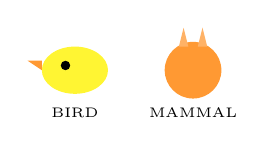
\begin{tikzpicture}[scale=0.6]
% Duck (bird)
\fill[yellow!80] (0,0) ellipse (0.7 and 0.5);
\fill[orange!80] (-0.7,0) -- (-1,0.2) -- (-0.7,0.2);
\fill[black] (-0.2,0.1) circle (0.1);
\node[below,font=\tiny] at (0,-0.6) {BIRD};

% Cat (mammal)
\fill[orange!80] (2.5,0) circle (0.6);
\fill[orange!60] (2.2,0.5) -- (2.3,0.9) -- (2.4,0.5);
\fill[orange!60] (2.8,0.5) -- (2.7,0.9) -- (2.6,0.5);
\node[below,font=\tiny] at (2.5,-0.6) {MAMMAL};
\end{tikzpicture}
\end{center}

\column{0.48\textwidth}
\textbf{ML Approach}

\textbf{Step 1: Learning (NO LABELS)}

\begin{center}
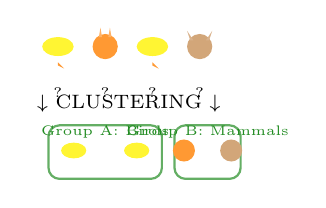
\begin{tikzpicture}[scale=0.4]
% Mixed animals with NO labels
\fill[yellow!80] (0,0) ellipse (0.5 and 0.3);
\fill[orange!80] (0,-0.5) -- (0.2,-0.7) -- (0,-0.6);
\node[below,font=\tiny] at (0,-1) {?};

\fill[orange!80] (1.5,0) circle (0.4);
\fill[orange!60] (1.3,0.3) -- (1.35,0.6) -- (1.4,0.3);
\fill[orange!60] (1.7,0.3) -- (1.65,0.6) -- (1.6,0.3);
\node[below,font=\tiny] at (1.5,-1) {?};

\fill[yellow!80] (3,0) ellipse (0.5 and 0.3);
\fill[orange!80] (3,-0.5) -- (3.2,-0.7) -- (3,-0.6);
\node[below,font=\tiny] at (3,-1) {?};

\fill[brown!70] (4.5,0) circle (0.4);
\fill[brown!60] (4.2,0.2) -- (4.1,0.5) -- (4.3,0.2);
\fill[brown!60] (4.8,0.2) -- (4.9,0.5) -- (4.7,0.2);
\node[below,font=\tiny] at (4.5,-1) {?};

\node[font=\scriptsize] at (2.25,-1.8) {$\downarrow$ CLUSTERING $\downarrow$};

% Discovered groups
\draw[thick,unsupervisedgreen!70,rounded corners] (-0.3,-2.5) rectangle (3.3,-4.2);
\node[font=\tiny,unsupervisedgreen] at (1.5,-2.7) {Group A: Birds};
\fill[yellow!80] (0.5,-3.3) ellipse (0.4 and 0.25);
\fill[yellow!80] (2.5,-3.3) ellipse (0.4 and 0.25);

\draw[thick,unsupervisedgreen!70,rounded corners] (3.7,-2.5) rectangle (5.8,-4.2);
\node[font=\tiny,unsupervisedgreen] at (4.75,-2.7) {Group B: Mammals};
\fill[orange!80] (4,-3.3) circle (0.35);
\fill[brown!70] (5.5,-3.3) circle (0.35);
\end{tikzpicture}
\end{center}

\vspace{0.2em}
\textbf{Step 2: Application}

\begin{center}
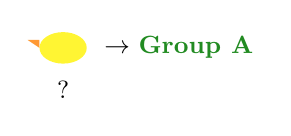
\begin{tikzpicture}[scale=0.5]
% New duck
\fill[yellow!80] (0,0) ellipse (0.6 and 0.4);
\fill[orange!80] (-0.6,0) -- (-0.9,0.2) -- (-0.6,0.2);
\node[below,font=\small] at (0,-0.6) {?};
\node[right,font=\small] at (0.8,0) {$\rightarrow$ \textcolor{unsupervisedgreen}{\textbf{Group A}}};
\end{tikzpicture}
\end{center}
\end{columns}

\bottomnote{Example: Algorithm discovers natural groupings based on visual features without being told what defines each category}
\end{frame}

% ==================== REINFORCEMENT EXAMPLE WITH DUCK ====================
\begin{frame}[t]{\textcolor{reinforcementorange}{Reinforcement Learning Example: Duck Learning to Swim}}
\begin{columns}[T]
\column{0.48\textwidth}
\textbf{Traditional Approach}

Expert programs instructions:
\begin{itemize}
\item Paddle left foot at angle 45 degrees
\item Then paddle right foot
\item Repeat every 0.5 seconds
\item Adjust for current
\end{itemize}

\vspace{0.3em}
\begin{center}
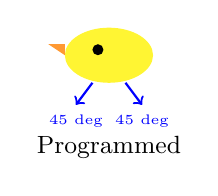
\begin{tikzpicture}[scale=0.7]
% Programmed duck with arrows showing movements
\fill[yellow!80] (0,0) ellipse (0.8 and 0.5);
\fill[orange!80] (-0.8,0) -- (-1.1,0.2) -- (-0.8,0.2);
\fill[black] (-0.2,0.1) circle (0.1);
\draw[->,thick,blue] (-0.3,-0.5) -- (-0.6,-0.9) node[below,font=\tiny] {45 deg};
\draw[->,thick,blue] (0.3,-0.5) -- (0.6,-0.9) node[below,font=\tiny] {45 deg};
\node[below,font=\small] at (0,-1.3) {Programmed};
\end{tikzpicture}
\end{center}

\column{0.48\textwidth}
\textbf{ML Approach}

\textbf{Step 1: Learning (Trial \& Error)}

\begin{center}
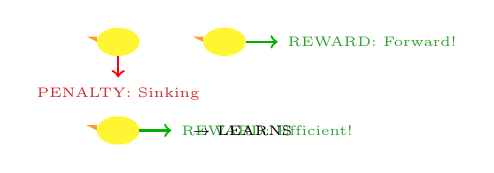
\begin{tikzpicture}[scale=0.45]
% Trial 1: Sinking (bad)
\fill[yellow!80] (0,0) ellipse (0.6 and 0.4);
\fill[orange!80] (-0.6,0) -- (-0.9,0.15) -- (-0.6,0.15);
\draw[->,thick,red] (0,-0.4) -- (0,-1) node[below,font=\tiny,text=mlred] {PENALTY: Sinking};

% Trial 2: Forward (good)
\fill[yellow!80] (3,0) ellipse (0.6 and 0.4);
\fill[orange!80] (2.4,0) -- (2.1,0.15) -- (2.4,0.15);
\draw[->,thick,green!70!black] (3.6,0) -- (4.5,0) node[right,font=\tiny,text=mlgreen] {REWARD: Forward!};

% Trial 3: Balanced (learning)
\fill[yellow!80] (0,-2.5) ellipse (0.6 and 0.4);
\fill[orange!80] (-0.6,-2.5) -- (-0.9,-2.35) -- (-0.6,-2.35);
\draw[->,thick,green!70!black] (0.6,-2.5) -- (1.5,-2.5) node[right,font=\tiny,text=mlgreen] {REWARD: Efficient!};
\node[font=\tiny] at (3.5,-2.5) {$\rightarrow$ LEARNS};
\end{tikzpicture}
\end{center}

\vspace{0.2em}
\textbf{Step 2: Deployment}

\begin{center}
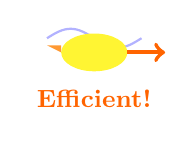
\begin{tikzpicture}[scale=0.6]
% Skilled duck swimming in waves
\draw[blue!30,thick] (0,0.3) sin (0.5,0.5) cos (1,0.3) sin (1.5,0.1) cos (2,0.3);
\fill[yellow!80] (1,0) ellipse (0.7 and 0.4);
\fill[orange!80] (0.3,0) -- (0,0.15) -- (0.3,0.15);
\draw[->,thick,reinforcementorange,line width=1.5pt] (1.7,0) -- (2.5,0);
\node[below,font=\small] at (1,-0.6) {\textcolor{reinforcementorange}{\textbf{Efficient!}}};
\end{tikzpicture}
\end{center}
\end{columns}

\bottomnote{Example: Duck learns optimal swimming through thousands of attempts, discovering techniques experts might never explicitly program}
\end{frame}

% ==================== MODEL EVALUATION ====================
\begin{frame}[t]{Model Evaluation: Understanding Overfitting}
\begin{columns}[T]
\column{0.58\textwidth}
\begin{center}
\includegraphics[width=0.98\textwidth,height=0.75\textheight,keepaspectratio]{learning_curves.pdf}
\end{center}

\column{0.38\textwidth}
\textbf{The Problem:}

\textcolor{mlred}{\textbf{Overfitting}}: Model memorizes training data, fails on new data

\textcolor{mlgreen}{\textbf{Good generalization}}: Small gap between train and validation error

\vspace{0.5em}
\textbf{Critical Rule:}

\textbf{NEVER evaluate on training data!}

Training accuracy is meaningless - can achieve 100\% by memorization.

\vspace{0.5em}
\textbf{Data Splits:}
\begin{itemize}
\item \textbf{Train} (70\%): Fit
\item \textbf{Val} (15\%): Tune
\item \textbf{Test} (15\%): Evaluate ONCE
\end{itemize}

\vspace{0.5em}
\textbf{Solutions:}
\begin{itemize}
\item More data
\item Regularization
\item Simpler model
\item Early stopping
\item Cross-validation
\end{itemize}
\end{columns}

\bottomnote{Watch validation error: if it increases while training error decreases, you're overfitting!}
\end{frame}

% ==================== EVALUATION METRICS ====================
\begin{frame}[t]{Evaluation Metrics \& Confusion Matrix}
\begin{columns}[T]
\column{0.52\textwidth}
\begin{center}
\includegraphics[width=0.95\textwidth,keepaspectratio]{confusion_matrix.pdf}
\end{center}

\column{0.44\textwidth}
\textbf{Classification Metrics:}
\begin{itemize}
\item \textbf{Accuracy}: Correct / Total

{\small (Can be misleading with imbalanced data!)}
\item \textbf{Precision}: TP / (TP + FP)

{\small How many predicted positives are actually positive?}
\item \textbf{Recall}: TP / (TP + FN)

{\small How many actual positives did we find?}
\item \textbf{F1 Score}: Harmonic mean of precision/recall
\item \textbf{ROC-AUC}: Trade-off curve
\end{itemize}

\vspace{0.5em}
\textbf{Regression Metrics:}
\begin{itemize}
\item MSE, RMSE, MAE
\item R$^2$: Explained variance (0-1)
\end{itemize}
\end{columns}

\bottomnote{Confusion matrix reveals which types of errors your model makes - essential for understanding performance}
\end{frame}

% ==================== COMMON PITFALLS ====================
\begin{frame}[t]{Common Pitfalls in Machine Learning}
\begin{columns}[T]
\column{0.48\textwidth}
\textbf{1. Data Leakage}

Information from test set ``leaks'' into training

\textcolor{mlred}{\textbf{Example:}} Normalizing before splitting data

\textbf{Result:} Artificially inflated performance

\vspace{0.5em}
\textbf{2. Overfitting}

Model too complex, memorizes training data

\textbf{Signs:} High train accuracy, low test accuracy

\textbf{Solutions:} Regularization, more data, simpler model, dropout

\vspace{0.5em}
\textbf{3. Selection Bias}

Training data not representative of real distribution

\textcolor{mlred}{\textbf{Example:}} Face recognition trained only on certain demographics

\textbf{Result:} Poor performance on underrepresented groups

\column{0.48\textwidth}
\textbf{4. Distribution Shift}

Test distribution differs from training

\textbf{Result:} Model degrades in production

\textbf{Solution:} Continuous monitoring and retraining

\vspace{0.5em}
\textbf{5. Ignoring Class Imbalance}

99\% accuracy meaningless if 99\% of data is one class

\textbf{Solutions:} Stratified sampling, weighted loss, SMOTE, use F1/AUC not accuracy

\vspace{0.5em}
\textbf{6. Not Using Baseline}

Always compare to simple baseline:
\begin{itemize}
\item Random guessing
\item Most frequent class
\item Simple rules
\end{itemize}

\textbf{If ML doesn't beat baseline significantly, don't use ML!}
\end{columns}

\bottomnote{Most ML failures come from data problems, not algorithm choice - focus on data quality and proper evaluation}
\end{frame}

% ==================== COLORFUL EXAMPLES ====================
\begin{frame}[t]{Real-World Applications}
\begin{columns}[T]
\column{0.31\textwidth}
\begin{center}
\textcolor{supervisedblue}{\textbf{\Large Supervised}}
\end{center}

\vspace{0.3em}
\colorbox{supervisedblue!10}{%
\begin{minipage}{0.95\columnwidth}
\textbf{\textcolor{supervisedblue}{Email Spam Filter}}
\begin{itemize}
\item Input: Email text
\item Label: Spam or Not Spam
\item Learn: Text patterns
\end{itemize}
\end{minipage}
}

\vspace{0.3em}
\colorbox{supervisedblue!10}{%
\begin{minipage}{0.95\columnwidth}
\textbf{\textcolor{supervisedblue}{Medical Diagnosis}}
\begin{itemize}
\item Input: Patient scans
\item Label: Disease present
\item Learn: Visual markers
\end{itemize}
\end{minipage}
}

\vspace{0.3em}
\colorbox{supervisedblue!10}{%
\begin{minipage}{0.95\columnwidth}
\textbf{\textcolor{supervisedblue}{Fraud Detection}}
\begin{itemize}
\item Input: Transaction data
\item Label: Fraudulent or legitimate
\item Learn: Fraud patterns (often semi-supervised)
\end{itemize}
\end{minipage}
}

\column{0.31\textwidth}
\begin{center}
\textcolor{unsupervisedgreen}{\textbf{\Large Unsupervised}}
\end{center}

\vspace{0.3em}
\colorbox{unsupervisedgreen!10}{%
\begin{minipage}{0.95\columnwidth}
\textbf{\textcolor{unsupervisedgreen}{Customer Segmentation}}
\begin{itemize}
\item Input: Purchase behavior
\item No labels needed
\item Find: Customer groups
\end{itemize}
\end{minipage}
}

\vspace{0.3em}
\colorbox{unsupervisedgreen!10}{%
\begin{minipage}{0.95\columnwidth}
\textbf{\textcolor{unsupervisedgreen}{Anomaly Detection}}
\begin{itemize}
\item Input: System logs, sensor data
\item No labels for anomalies
\item Find: Unusual patterns
\end{itemize}
\end{minipage}
}

\vspace{0.3em}
\colorbox{unsupervisedgreen!10}{%
\begin{minipage}{0.95\columnwidth}
\textbf{\textcolor{unsupervisedgreen}{Topic Modeling}}
\begin{itemize}
\item Input: Document text
\item No topic labels
\item Find: Hidden themes
\end{itemize}
\end{minipage}
}

\column{0.31\textwidth}
\begin{center}
\textcolor{reinforcementorange}{\textbf{\Large Reinforcement}}
\end{center}

\vspace{0.3em}
\colorbox{reinforcementorange!10}{%
\begin{minipage}{0.95\columnwidth}
\textbf{\textcolor{reinforcementorange}{Game AI (AlphaGo)}}
\begin{itemize}
\item State: Board position
\item Action: Move choice
\item Reward: Win or lose
\end{itemize}
\end{minipage}
}

\vspace{0.3em}
\colorbox{reinforcementorange!10}{%
\begin{minipage}{0.95\columnwidth}
\textbf{\textcolor{reinforcementorange}{Autonomous Vehicles}}
\begin{itemize}
\item State: Road conditions
\item Action: Steering, speed
\item Reward: Safe driving
\end{itemize}
\end{minipage}
}

\vspace{0.3em}
\colorbox{reinforcementorange!10}{%
\begin{minipage}{0.95\columnwidth}
\textbf{\textcolor{reinforcementorange}{Robot Control}}
\begin{itemize}
\item State: Robot position
\item Action: Motor commands
\item Reward: Task success
\end{itemize}
\end{minipage}
}
\end{columns}

\bottomnote{Each paradigm excels at different types of problems}
\end{frame}

% ==================== COMPARISON ====================
\begin{frame}[t]{Paradigm Comparison}
\begin{table}
\centering
\small
\begin{tabular}{p{2.5cm}p{3.5cm}p{3.5cm}p{3.5cm}}
\toprule
\textbf{Aspect} & \textcolor{supervisedblue}{\textbf{Supervised}} & \textcolor{unsupervisedgreen}{\textbf{Unsupervised}} & \textcolor{reinforcementorange}{\textbf{Reinforcement}} \\
\midrule
\textbf{Data} & Labeled examples & Unlabeled data & Environment interaction \\
\midrule
\textbf{Feedback} & Correct answers provided & No explicit feedback & Rewards/penalties \\
\midrule
\textbf{Goal} & Predict outputs for new inputs & Discover structure in data & Learn optimal policy \\
\midrule
\textbf{Common Use} & Classification, regression & Clustering, dimensionality reduction & Control, decision making \\
\midrule
\textbf{Challenges} & Requires labeled data & Evaluation difficulty & Training complexity \\
\midrule
\textbf{Examples} & Image recognition, spam detection & Customer segmentation, anomaly detection & Game AI, robotics \\
\bottomrule
\end{tabular}
\end{table}

\vspace{0.5em}
\textbf{Choosing the Right Paradigm:}
\begin{itemize}
\item \textcolor{supervisedblue}{\textbf{Supervised}}: When you have labeled data and clear target outputs
\item \textcolor{unsupervisedgreen}{\textbf{Unsupervised}}: When you want to explore data and find hidden patterns
\item \textcolor{reinforcementorange}{\textbf{Reinforcement}}: When learning through sequential decisions and feedback
\end{itemize}

\bottomnote{Modern AI often combines multiple paradigms for optimal results}
\end{frame}

% ==================== KEY INSIGHTS ====================
\begin{frame}[t]{Key Insights}
\begin{columns}[T]
\column{0.48\textwidth}
\textbf{Traditional vs ML}

The fundamental shift:
\begin{itemize}
\item Traditional: \textbf{Rules first}, then apply to data
\item ML: \textbf{Data first}, then learn rules
\end{itemize}

\vspace{0.5em}
\textbf{When Traditional Methods Work Best:}
\begin{itemize}
\item Well-defined, stable rules
\item High interpretability required
\item Limited data available
\item Regulatory compliance critical
\end{itemize}

\column{0.48\textwidth}
\textbf{The ML Advantage}

Why ML excels:
\begin{itemize}
\item Handles complex, high-dimensional patterns
\item Adapts to changing environments
\item Scales with data availability
\item Discovers non-obvious relationships
\end{itemize}

\vspace{0.5em}
\textbf{Critical Considerations:}
\begin{itemize}
\item \textbf{Data quality > quantity}: Garbage in, garbage out
\item \textbf{Bias in data = bias in model}: Training data must be representative
\item \textbf{Interpretability crisis}: Complex models are black boxes
\item \textbf{Maintenance burden}: Models degrade, need monitoring and retraining
\item \textbf{Cold start problem}: ML needs data to begin
\end{itemize}
\end{columns}

\vspace{0.5em}
\textbf{Ethical and Practical Concerns:}
\begin{itemize}
\item \textbf{Fairness}: Biased training data leads to discriminatory models (e.g., hiring, lending, criminal justice)
\item \textbf{Privacy}: ML often requires large datasets - data governance critical
\item \textbf{When NOT to use ML}: Simple rules work, need explainability, insufficient data, high-stakes decisions requiring guarantees
\end{itemize}

\vspace{0.5em}
\begin{center}
\colorbox{mllavender4}{%
\begin{minipage}{0.9\textwidth}
\centering
\textbf{Best Practice:} Start simple with traditional methods, explore ML when complexity + data justify it, and always prioritize data quality over algorithm choice
\end{minipage}
}
\end{center}

\bottomnote{Success in ML depends more on data quality, problem formulation, and evaluation strategy than on algorithm selection}
\end{frame}

% ==================== SUMMARY ====================
\begin{frame}[plain]
\vspace{2cm}
\begin{center}
{\Huge Summary}\\[1cm]
{\Large Machine Learning offers three powerful paradigms:}\\[0.7cm]
{\large \textcolor{supervisedblue}{\textbf{Supervised}} - Learn from labeled examples}\\
{\large \textcolor{unsupervisedgreen}{\textbf{Unsupervised}} - Discover hidden patterns}\\
{\large \textcolor{reinforcementorange}{\textbf{Reinforcement}} - Learn through interaction}\\[1.5cm]
{\normalsize Each excels at different types of problems}\\
{\normalsize Choose based on your data, goals, and constraints}\\[1.5cm]
{\normalsize Questions?}
\end{center}
\end{frame}

\end{document}
